\section{Feature Representation} \label{sec:chp2-sec4}
The previous section described why there is a need for feature extraction.
This section discusses the reasons behind feature representation.
%we explained the need for feature extraction, in this section we discuss why there is a need for feature representation.

The ``Curse of dimensionality''(correlated and irrelevant features)~\cite{Theodoridis2006327} has always been a challenge in the field of classification and pattern recognition. 
Besides, high computational cost and over-fitting, learning with irrelevant features reduces the precision and performance of the system, hence, it is essential to learn the most representative and uncorrelated features.  
%Creating a new feature space either by reducing the original dimensionality to more representative, uncorrelated dimensions or by modeling it into a new feature space defines our idea of feature representation. 
The goal of feature representation is to create a new feature space either by reducing the original dimensionality to more representative and uncorrelated dimensions, or by modelling it into a new feature sapce.

\acf{sffs}, \acf{sbfs} \cite{ferri1994comparative}, and \acf{mrmr}~\cite{peng2005feature} are feature selection methods that pick only the most relevant feature dimensions from the original space.
\acf{lda}~\cite{martinez2001pca} and \ac{pca} are linear dimension reduction approaches, that linearly project data into a new subspace with lower dimensionality. 
Linear mapping of the data is not always achievable and in some cases, nonlinear projection of the feature space to lower subspaces is required.
Kernel \ac{pca} (non-linear \ac{pca})~\cite{mika1998kernel} is one of the methods used for non-linear mapping, among others.
%Nonlinear projections of the feature space to lower subspace is possible through kernel \ac{pca} (nonlinear \ac{pca}), \acf{mvu}, and  \acf{lle} among others.

The aforementioned methods reduce the dimensionality in one way or another, however, there are other approaches that can map feature space to a new separable space, e.g. \acf{bow} and \ac{scf}.
The former tries to find similar patterns in the feature space and perform the mapping based on their clusters (``visual words'').
The latter maps the feature space to a sparse space in which each sample is defined by a set a of few elements. 
A more detailed explanation of the above methods is presented in the following.

\begin{description}
\item \textbf{Sequential Forward/Backward Feature Selection (\ac{sffs}/\ac{sbfs})} are greedy algorithms that start with an empty or full set and sequentially add or remove the best or worst features to the set, respectively.
These suboptimal methods obtain a chain of nested subsets of features~\cite{ferri1994comparative}.
Nested subsets are the main drawback of these approaches, since once a feature set is added or subtracted, it can not be discarded or retained.

\item \textbf{\acf{mrmr}} is another feature selection approach that chooses attributes maximizing their relevance to or dependency on the distribution to a target class $c$, while keeping their redundancy to a minimum~\cite{peng2005feature}.
This technique is based on the idea that ``the $m$ best features are not the best $m$ features'', meaning that, besides selecting the best relevant features, we have to make sure that they are not highly dependent on each other. 

The relevance of a feature set is a measure of its efficacy with respect to the target class.
In simple terms, it determines how well a variable discriminates between classes~\cite{auffarth2010comparison}, which makes it a measure between the feature and the class. 
%Thus it is a measure between the feature and the class.
Several criteria can be used to measure the relevance of a feature set such as correlation and mutual information, among others~\cite{auffarth2010comparison}. 
Redundancy criteria measures the similarity between the attributes distribution in order to find mutually exclusive features. 
Similar to relevance, different criteria can be used to measure redundancy (e.g., redundancy fit criterion and sign test)~\cite{auffarth2010comparison}.

\item \textbf{\acf{lda}} (also called Fisher Discriminant Analysis) applies a supervised linear transformation to map the original space to a new one with a low dimensionality.
This approach searches for the subspaces in the underlying space that best discriminates between classes rather than those that best describe the data~\cite{martinez2001pca}. 
Considering a feature space, \ac{lda} creates a linear combination of independent features while preserving the largest mean difference between the desired classes and minimum mean distance within each classes. 
Formulating the problem, two measures are defined: (1) within-class scatter matrix, given by
$$ S_{w} = \sum\limits_{j=1}^{c}\sum\limits_{i=1}^{N_{j}}(x_{i}^{j}-\mu_{j})(x_{i}^{j}-\mu_{j})^{T},$$
\noindent where $x_{i}^{j}$ is the $i^{th}$ sample of class $j$, $\mu_{j}$ is the mean of class j, $N_{j}$ the number of samples in class $j$ and $C$ the number of classes.\\
\noindent(2) between-class scatter matrix, give by  
$$ S_{b} = \sum\limits_{j=1}^{c}(\mu_{j}-\mu)(\mu_{j}-\mu)^{T}, $$
where $\mu$ represents the mean of all the classes.
The final goal is to maximize the between-class measure ($S_{b}$) while minimizing the within-class distance ($S_{w}$). 
This is possible by maximizing the ratio $det\vert S_{b}\vert / det\vert S_{w}\vert$~\cite{martinez2001pca}.

\item \textbf{\Acf{pca}} is an unsupervised orthogonal linear transformation approach intended to search out subspaces in which the variation of the data is maximized. 
The transformed subspace by \ac{pca} is a new orthogonal uncorrelated coordinate system.
\ac{pca} transforms the data into a new coordinate system where the greatest data variance is along the first coordinate, the second greatest variance is along the second coordinate and so on. 
The data variation in the new coordinate system is modeled by eigenvalues $\lambda_{i}$  along their associated eigenvectors $e_{i}$.
In simpler terms, the coordinates of the new systems are defined by the eigenvectors (also called principal components).
Considering $W$ as an orthogonal linear transformation model that maps the original $D$-dimensional space to a $d$-dimensional space ($d \le D$), the new space $Y$ is defined by: 
\begin{equation}
Y = W^{T}X~.
\end{equation}
\noindent The transformation matrix $W$ is constructed by eigenvectors $e_{i}$ (each column of $W$ corresponds to one eigenvector) of the covariance or scatter matrix of the data ($ S = XX^{T}$). 
\begin{equation}
\lambda e = Se~.
\end{equation}
Using \ac{pca}, the dimensionality of the data can be reduced by considering only the first principal components. 
In doing so, the dimensionality of the data is reduced while maximal variance of the original data is preserved. 
\ac{pca} is scale sensitive, thus data normalization is crucial.
The data should also be mean-subtracted to assure that the eigenvector with the highest eigenvalues is along the maximum variance, and not the mean of the data.

\item \textbf{Kernel \ac{pca}} is a nonlinear, unsupervised transformation that assumes that the features are mapped with a nonlinear transformation $\phi(x)$ to a new $M$-dimensions feature space ($M$ could be much higher than the original data space $D$).
By using this transformation, each point $x_{n}$ is projected onto a point $\phi(x_{n})$. 
The idea of the kernel \ac{pca} is to perform a standard \ac{pca} in the feature space rather than the data space, which will create nonlinear principal components in the original data space (see Fig.~\ref{fig:kpca}).
\begin{figure}
\centering
\subfloat[]{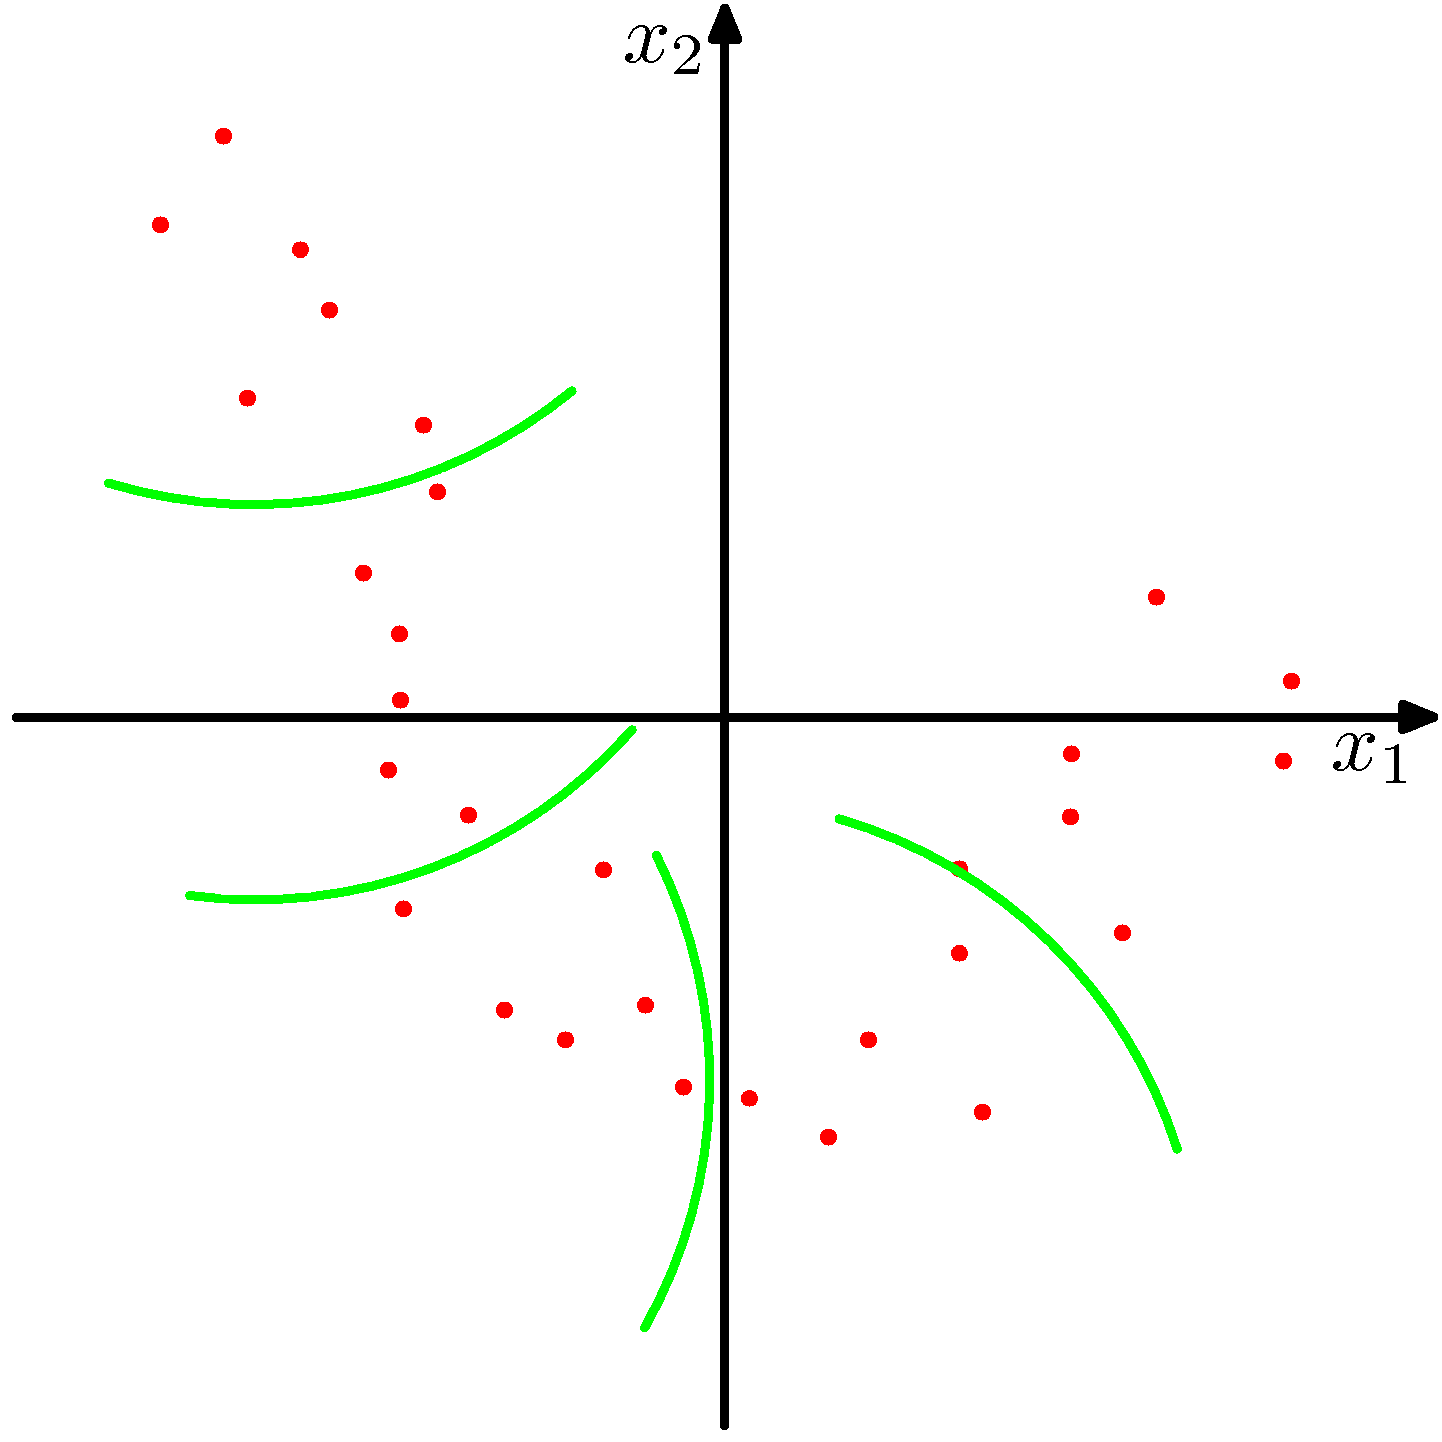
\includegraphics[width = 0.45\textwidth]{Chapter2/Figures/Figure12_16a.png}}\hfill
\subfloat[]{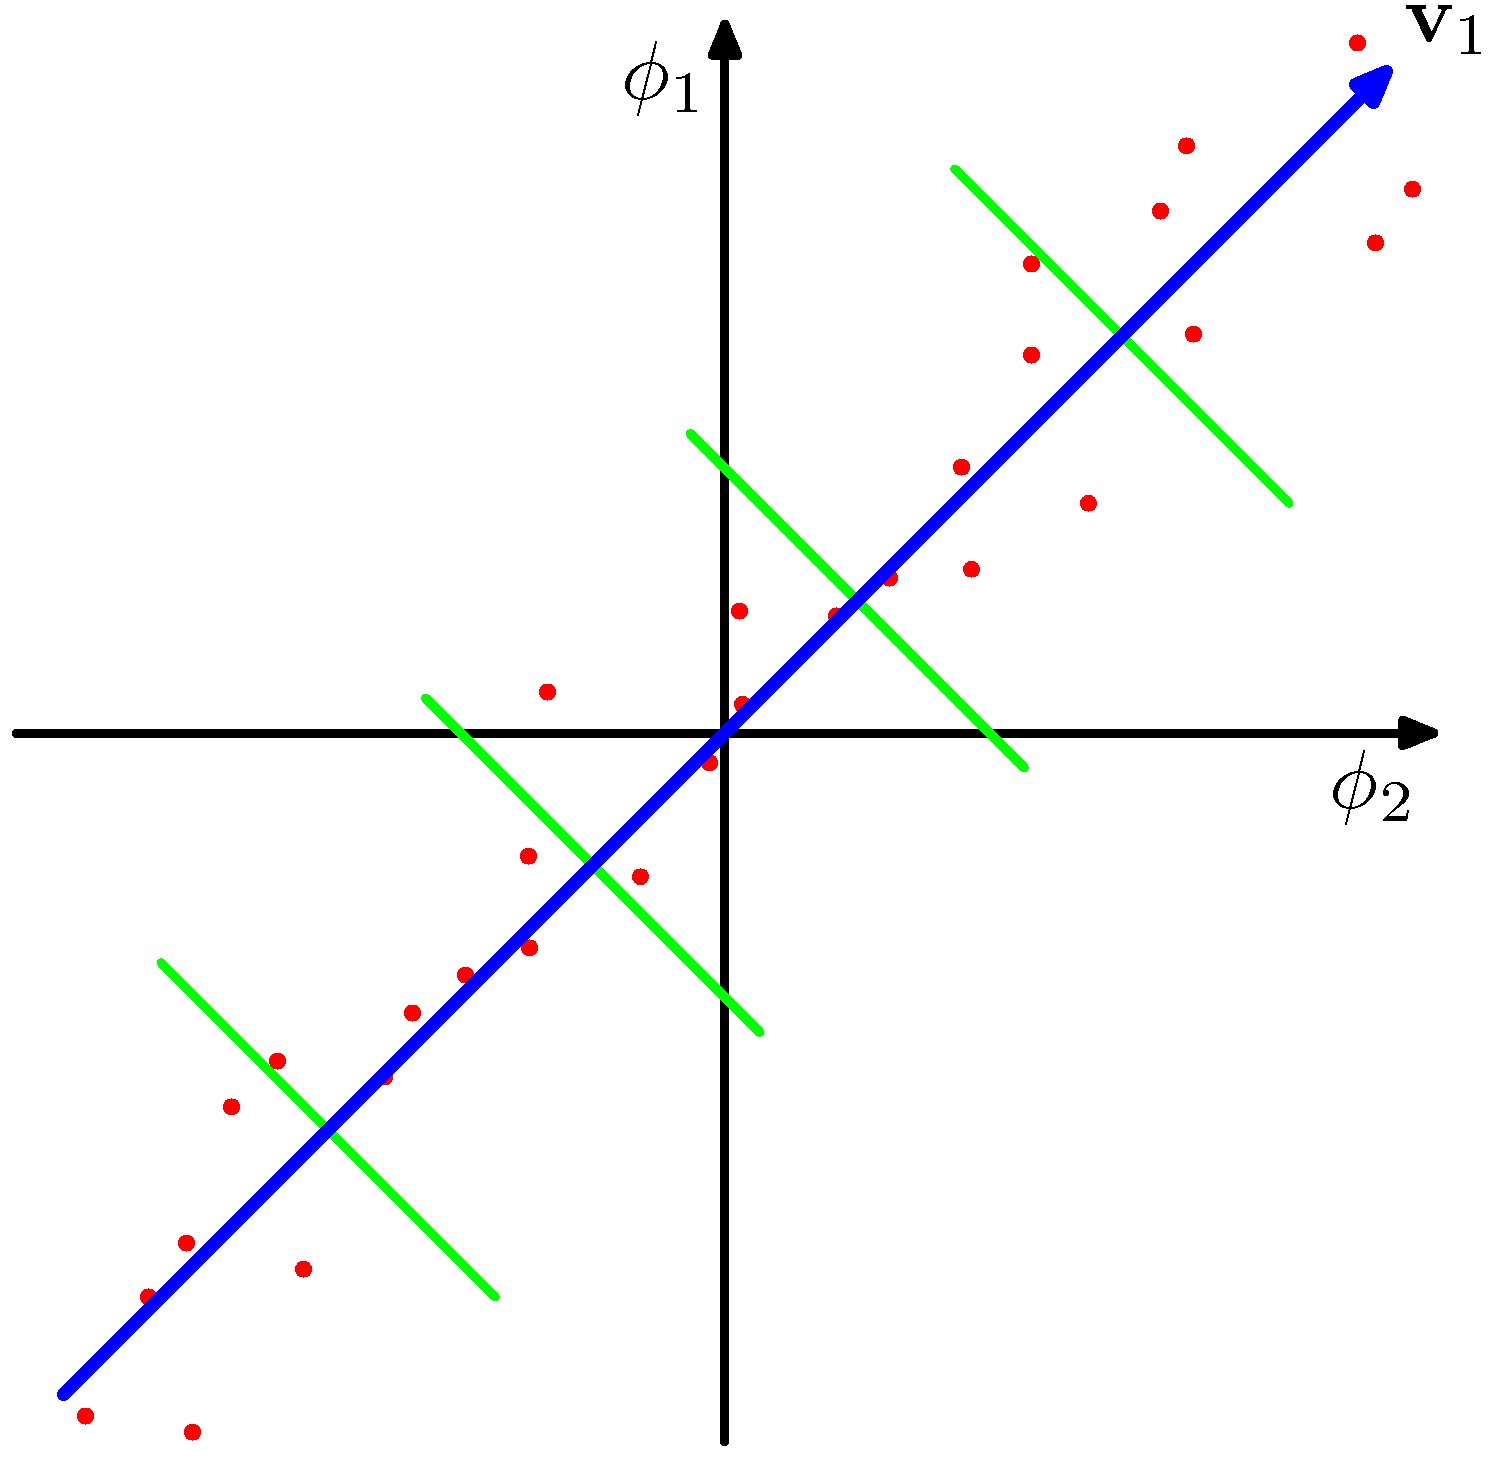
\includegraphics[width = 0.45\textwidth]{Chapter2/Figures/Figure12_16b.png}}
\caption[Kernel \ac{pca}]{Illustration of kernel \ac{pca}. (a) Nonlinear principal component in the original data space, (b) Nonlinear projection of the original data space into features space ($\phi(x)$).
In this space it is possible to apply linear \ac{pca}, $v_{1}$ is the first principal component in the feature space and the green lines are linear projections of the data to the principal component. This figure was taken from Bishop~et al.\,\cite{bishop2006pattern}.}
\label{fig:kpca}
\end{figure}   
Assuming that the projected data in the feature space is zero-mean, the covariance matrix in the feature space is given by: 
\begin{equation}
C_{M \times M} = \frac{1}{N}\sum\limits_{n=1}^{N} \phi(x_{n})\phi(x_{n})^{T}~.
\label{eq:Covkpca}
\end{equation}
Similar to the standard \ac{pca}, our goal is to find the eigenvectors of this matrix where the eigendecomposition is given by: 
\begin{equation}
\lambda_{i} v_{i} = C v_{i}.
\label{eq:edeckpca}
\end{equation}
Substituting Eq.~\ref{eq:Covkpca} in Eq.~\ref{eq:edeckpca}, the eigenvectors are given by: 
\begin{equation}
v_{i} = \sum_{n=1}^{N} a_{in}\phi(x_{n}).
\end{equation}
Using the previous formulation in the eigendecomposition, and based on the kernel substitution, the mapping in the feature space can be represented in terms of a kernel function $k(x_{n}, x_{m})$: 
\begin{subequations}
\begin{align}
\frac{1}{N}\sum\limits_{n=1}^{N} k(x_{l}, x_{n}) \sum\limits_{m=1}^{N} a_{im}k(x_{n}, x_{m}) & = \lambda_{i} \sum\limits_{n=1}^{N} a_{in}k(x_{l}, x_{n})~,\\
K a_{i} & = \lambda_{i}N a_{i},
\end{align}
\end{subequations} 
\noindent Here $a_{i}$ is an $N$-dimensional vector and $K$ is an $N \times N$ matrix solved by eigenvalue decomposition.
Based on the aforementioned equations, we can now formulate the principal component projections in terms of the kernel function as illustrated below: 
\begin{equation}
y_{i}(x) = \phi(x)^{T}v_{i} = \sum\limits_{n =1}^{N} a_{in}\phi(x)^{T}\phi(x_{n}) = \sum\limits_{n=1}^{N} a_{in}k(x,x_{n})~.
\end{equation} 

%\item \textbf{\acf{mvu}}
%\item \textbf{\acf{lle}}

\item \textbf{\acf{bow}} is a modeling or mapping of the extracted features to a new space based on a set of main clusters in the feature space. 
This method looks for similar or strong patterns among the extracted features and presents all the features based on the number of occurrence of these patterns. 
\Ac{bow} clusters a set of low-level features using a \textit{k}-means algorithm to create a ``codebook'' of ``visual words''.
Each visual word is defined by a centroid of the corresponding cluster. 
After creating the codebook, each sample is represented as a histogram of size \textit{k} obtained by calculating the occurrence frequency of the \textit{k} words among the features extracted from the sample.

K-means is an iterative algorithm that finds k centroids by alternating assignment and update steps.
The assignment steps are based on $L_{2}$ norm (Euclidean) distance.
Different initialization methods can be used in order to assign the initial \textit{k} clusters~\cite{celebi2013comparative}.
In this research, these clusters are selected based on the greedy \textit{k}-means++ method~\cite{arthur2007k}.
The choice of the visual words (number of \textit{k} clusters) depends on the application, and different choices can be made. 
A suitable number is usually found via an exhaustive search or primary tests.  


\item \textbf{\acf{scf}}, or sparse signal representation, has become very popular over the past few decades and has led to state-of-the-art results in various applications such as face recognition~\cite{wright2009robust}, image denoising, image inpainting~\cite{elad2006image}, and image classification~\cite{sidibe2015discrimination}. 
The main goal of sparse modeling is to efficiently represent the samples/images as a linear combination of a few typical patterns, called atoms, selected from the dictionary.
Sparse coding consists of three main steps: (i) dictionary learning, (ii) low-level feature projection, and (iii) feature pooling~\cite{rubinstein2008efficient}. 
Considering our dictionary $D \in R^{n \times K}$ with $K$ atoms, where each column of $D$ represents one atom, the sparse coding problem of a signal $y \in R^{n}$ is defined as finding the sparsest vector $x$ so that $y \approx Dx$. 
This is an optimization problem that can be formulated as:
\begin{equation}
\min_{x} \|y-Dx\|_{2} \qquad \text{s.t.}\ \|x\|_{0} \leq \lambda \,,
\end{equation}  
\noindent where $\lambda$ is the sparsity level and $l^{0}$-norm accounts for the minimum number of non-zero elements in the sparse vector $x$. 
This optimization problem is NP hard~\cite{Elad2010}, subsequently approximation solutions are proposed either by using greedy algorithms such as \ac{mp}~\cite{mallat1993matching} and \ac{omp}~\cite{davis1994adaptive}, or by replacing the $l^{0}$-norm with $l^{1}$-norm such as in the \ac{bp} algorithm~\cite{chen1998atomic}.
%\noindent where $\lambda$ is the sparsity level and $l^{0}$-norm accounts for the minimum number of non-zero elements in sparse vector $x$. 
%This optimization problem is NP hard~\cite{Elad2010}.
%Subsequently approximation solutions are proposed either by using greedy algorithms such as \ac{mp}~\cite{mallat1993matching} and \ac{omp}~\cite{davis1994adaptive} or by replacing the $l^{0}$-norm with $l^{1}$-norm such as \ac{bp}~\cite{chen1998atomic}.
The dictionary is learned using K-SVD, a generalized version of \textit{k}-means clustering that uses \ac{svd}~\cite{aharon2006img}. 
The dictionary is built such that:
\begin{equation}
  \min_{Dx} \|y - Dx\|_{2} \qquad  \text{s.t.} \ \forall i \ \|x_{i}\|_{1} \leq \lambda \,,
\end{equation}

\noindent where $y$ is a low-level descriptor, $x$ is the sparse coded descriptor (i.e., high-level descriptor) with a sparsity level $\lambda$, and $D$ is the dictionary with $K$ atoms.
The K-SVD algorithm solves the optimization problem iteratively by alternating between $x$ and $D$. 
With $D$, the sparse code matrix $x$ is computed by any of the pursuit algorithms, and with $x$, $D$ is updated one atom at a time using \ac{svd}. 

Once the dictionary is learned, each $y_{i} \in R^{n}$ signal can be projected using $D$ to form a set of sparse codes $x_{i} \in R^{K}$. 
In the case of image samples, the sparse representation can be generated for patches in the image.
In this case, the final mapping is based on a combination of sparse codes, for instance by taking the maximum code from all the patches: 
\begin{equation}
f_{i} = \max_{j}(\vert X_{l}(i,j)\vert) \qquad  \forall  i = 1, 2, .., K \,,
\end{equation} 
\noindent where $X_{l} \in R^{K \times P}$ is the sparse code matrix~\cite{sidibe2015discrimination}. 
\end{description}



%In this research we choose, feature representation approaches such as \ac{pca}, \ac{bow}, and \ac{scf}. 



%%% Local Variables: 
%%% mode: latex
%%% TeX-master: "../thesis"
%%% End: 
